\documentclass{beamer}
\usepackage[utf8]{inputenc}

\usetheme{Madrid}
\usecolortheme{default}
\usepackage{amsmath,amssymb,amsfonts,amsthm}
\usepackage{txfonts}
\usepackage{tkz-euclide}
\usepackage{listings}
\usepackage{adjustbox}
\usepackage{array}
\usepackage{tabularx}
\usepackage{gvv}
\usepackage{lmodern}
\usepackage{circuitikz}
\usepackage{tikz}
\usepackage{graphicx}

\setbeamertemplate{page number in head/foot}[totalframenumber]

\usepackage{tcolorbox}
\tcbuselibrary{minted,breakable,xparse,skins}



\definecolor{bg}{gray}{0.95}
\DeclareTCBListing{mintedbox}{O{}m!O{}}{%
  breakable=true,
  listing engine=minted,
  listing only,
  minted language=#2,
  minted style=default,
  minted options={%
    linenos,
    gobble=0,
    breaklines=true,
    breakafter=,,
    fontsize=\small,
    numbersep=8pt,
    #1},
  boxsep=0pt,
  left skip=0pt,
  right skip=0pt,
  left=25pt,
  right=0pt,
  top=3pt,
  bottom=3pt,
  arc=5pt,
  leftrule=0pt,
  rightrule=0pt,
  bottomrule=2pt,
  toprule=2pt,
  colback=bg,
  colframe=orange!70,
  enhanced,
  overlay={%
    \begin{tcbclipinterior}
    \fill[orange!20!white] (frame.south west) rectangle ([xshift=20pt]frame.north west);
    \end{tcbclipinterior}},
  #3,
}
\lstset{
    language=C,
    basicstyle=\ttfamily\small,
    keywordstyle=\color{blue},
    stringstyle=\color{orange},
    commentstyle=\color{green!60!black},
    numbers=left,
    numberstyle=\tiny\color{gray},
    breaklines=true,
    showstringspaces=false,
}
%------------------------------------------------------------
%This block of code defines the information to appear in the
%Title page
\title %optional
{5.5.1}
\date{}
%\subtitle{A short story}

\author % (optional)
{Sai Krishna Bakki - EE25BTECH11049}

\begin{document}
\frame{\titlepage}
\begin{frame}{Question}
If $\vec{A}=\myvec{5&-1&4\\2&3&5\\5&-2&6}$, find $\vec{A}^{-1}$ and use it to solve the following system of equations
\begin{align*}
    5x-y+4z=5\\
    2x+3y+5z=2\\
    5x-2y+6z=-1
\end{align*}
\end{frame}

\begin{frame}{Theoretical Solution}
    \begin{align}
        \augvec{3}{3}{5&-1&4& 1& 0&0\\ 2&3&5& 0& 1&0\\5&-2&6& 0& 0&1}
        &\xleftrightarrow{\,R_3 \gets R_3 - R_1}
        \augvec{3}{3}{5&-1&4& 1& 0&0\\ 2&3&5& 0& 1&0\\0&-1&2& -1& 0&1} \end{align}
        \begin{align}
        &\xleftrightarrow[\,R_2 \gets R_2 + 3R_3]{\,R_1 \gets R_1 - R_3}
        \augvec{3}{3}{5&0&2& 2& 0&-1\\ 2&0&11& -3& 1&3\\0&-1&2& -1& 0&1}\end{align}
        \begin{align}
        &\xleftrightarrow{\,R_3 \gets -R_3}
        \augvec{3}{3}{5&0&2& 2& 0&-1\\ 2&0&11& -3& 1&3\\0&1&-2& 1& 0&-1} 
\end{align}
\end{frame}
\begin{frame}{Theoretical Solution}
    \begin{align}
        &\xleftrightarrow{\,R_2 \leftrightarrow R_3}
        \augvec{3}{3}{5&0&2& 2& 0&-1\\ 0&1&-2& 1& 0&-1\\2&0&11& -3& 1&3} \end{align}
        \begin{align}
        &\xleftrightarrow{\,R_1 \gets \frac{1}{5}R_1}
        \augvec{3}{3}{1&0&2/5& 2/5& 0&-1/5\\ 0&1&-2& 1& 0&-1\\2&0&11& -3& 1&3} \end{align}
        \begin{align}
        &\xleftrightarrow{\,R_3 \gets R_3 - 2R_1}
        \augvec{3}{3}{1&0&2/5& 2/5& 0&-1/5\\ 0&1&-2& 1& 0&-1\\0&0&51/5& -19/5& 1&17/5} \end{align}
\end{frame}
\begin{frame}{Theoretical Solution}
    \begin{align}
        &\xleftrightarrow{\,R_3 \gets \frac{5}{51}R_3}
        \augvec{3}{3}{1&0&2/5& 2/5& 0&-1/5\\ 0&1&-2& 1& 0&-1\\0&0&1& -19/51& 5/51&17/51} \end{align}
        \begin{align}
        &\xleftrightarrow[\,R_2 \gets R_2 + 2R_3]{\,R_1 \gets R_1 - \frac{2}{5}R_3}
        \augvec{3}{3}{1 & 0 & 0 & 28/51 & -2/51 & -17/51 \\ 0 & 1 & 0 & 13/51 & 10/51 & -17/51 \\ 0 & 0 & 1 & -19/51 & 5/51 & 17/51}
    \end{align}
    \begin{align}
        \therefore \vec{A}^{-1} = \myvec{ 28/51 & -2/51 & -17/51 \\ 13/51 & 10/51 & -17/51 \\ -19/51 & 5/51 & 17/51 }
    \end{align}
\end{frame}
\begin{frame}{Theoretical Solution}
    Now, Finding system of equations
\begin{align}
    \vec{A}\vec{X}=\vec{C}
\end{align}
where $\vec{C}=\myvec{5\\2\\-1}$ and $\vec{X}=\myvec{x\\y\\z}$
\begin{align}
    \vec{X}=\vec{A}^{-1}\vec{C}\\
    \vec{X}=\myvec{ 28/51 & -2/51 & -17/51 \\ 13/51 & 10/51 & -17/51 \\ -19/51 & 5/51 & 17/51 }\myvec{5\\2\\-1}\\
    \therefore \vec{X}=\myvec{3\\2\\-2}
\end{align}
\end{frame}
\begin{frame}[fragile]
\frametitle{C Code}
\begin{lstlisting}
#include <stdio.h>

// This function will be called from Python.
// It takes three integer values as arguments.
void process_point(int x, int y, int z) {
    // Print a confirmation message to the console.
    printf("✅ C function received point: (%d, %d, %d)\n", x, y, z);
}
\end{lstlisting}
\end{frame}
\begin{frame}[fragile]
\frametitle{Python Through Shared Output}
\begin{lstlisting} 
import ctypes
import subprocess
import os
import platform
import numpy as np
import matplotlib.pyplot as plt
from matplotlib.lines import Line2D

# --- Part 1: Calculate the Solution using NumPy ---

# Define the coefficient matrix A and the constant vector B
A = np.array([
    [5, -1, 4],
    [2,  3, 5],
    [5, -2, 6]
])
B = np.array([5, 2, -1])

# Use numpy.linalg.solve() to find the intersection point
\end{lstlisting}
\end{frame}
\begin{frame}[fragile]
\frametitle{Python Through Shared Output}
\begin{lstlisting} 

try:
    solution = np.linalg.solve(A, B)
    x_int, y_int, z_int = solution
    print(f"�� Python calculated intersection point: ({x_int:.0f}, {y_int:.0f}, {z_int:.0f})")
except np.linalg.LinAlgError:
    print("The system of equations has no unique solution.")
    exit()


# --- Part 2: Compile and Call C Function using ctypes ---

c_source_file = "points.c"
if platform.system() == "Windows":
    lib_file = "points.dll"
else:
    lib_file = "points.so"
\end{lstlisting}
\end{frame}
\begin{frame}[fragile]
\frametitle{Python Through Shared Output}
\begin{lstlisting} 
try:
    # Compile the C code into a shared library
    subprocess.run(["gcc", "-shared", "-o", lib_file, "-fPIC", c_source_file], check=True)
    
    # Load the shared library
    c_lib = ctypes.CDLL(os.path.join(os.getcwd(), lib_file))

    # Define the argument types for the C function (three integers)
    c_lib.process_point.argtypes = [ctypes.c_int, ctypes.c_int, ctypes.c_int]
    c_lib.process_point.restype = None

    # Call the C function, passing the values calculated by NumPy
    # We convert them to standard Python integers first
    c_lib.process_point(int(x_int), int(y_int), int(z_int))
\end{lstlisting}
\end{frame}
\begin{frame}[fragile]
\frametitle{Python Through Shared Output}
\begin{lstlisting} 
except (Exception) as e:
    print(f"An error occurred during C interaction: {e}")
    exit()


# --- Part 3: Generate the 3D Plot ---

def plane1(x, y): return (5 - 5*x + y) / 4
def plane2(x, y): return (2 - 2*x - 3*y) / 5
def plane3(x, y): return (-1 - 5*x + 2*y) / 6

x_grid, y_grid = np.meshgrid(np.linspace(-2, 8, 20), np.linspace(-2, 8, 20))
z1 = plane1(x_grid, y_grid)
z2 = plane2(x_grid, y_grid)
z3 = plane3(x_grid, y_grid)

fig = plt.figure(figsize=(10, 8))
ax = fig.add_subplot(111, projection='3d')
\end{lstlisting}
\end{frame}
\begin{frame}[fragile]
\frametitle{Python Through Shared Output}
\begin{lstlisting} 
ax.plot_surface(x_grid, y_grid, z1, alpha=0.6, color='red')
ax.plot_surface(x_grid, y_grid, z2, alpha=0.6, color='green')
ax.plot_surface(x_grid, y_grid, z3, alpha=0.6, color='blue')
ax.scatter(x_int, y_int, z_int, color='black', s=150, ec='white', zorder=10)

ax.set_xlabel('X-axis')
ax.set_ylabel('Y-axis')
ax.set_zlabel('Z-axis')
ax.set_title('Planes Intersecting at a Point Calculated by Python')

legend_elements = [
    Line2D([0], [0], color='red', lw=4, label='5x - y + 4z = 5'),
    Line2D([0], [0], color='green', lw=4, label='2x + 3y + 5z = 2'),
    Line2D([0], [0], color='blue', lw=4, label='5x - 2y + 6z = -1'),
    \end{lstlisting}
\end{frame}
\begin{frame}[fragile]
\frametitle{Python Through Shared Output}
\begin{lstlisting} 
    Line2D([0], [0], marker='o', color='w', markerfacecolor='black', markersize=10, label=f'Intersection: ({x_int:.0f}, {y_int:.0f}, {z_int:.0f})')
]
ax.legend(handles=legend_elements)

plt.show()
 \end{lstlisting}
\end{frame}
\begin{frame}[fragile]
\frametitle{Python Code}
\begin{lstlisting} 
import numpy as np
import matplotlib.pyplot as plt
from matplotlib.lines import Line2D

# --- Calculations based on the image ---

# Define the matrices A and B from the system of equations AX = B
A = np.array([
    [5, -1, 4],
    [2, 3, 5],
    [5, -2, 6]
])

B = np.array([5, 2, -1])

# Calculate the inverse of A and the solution X
# X = [x, y, z]
try:
    A_inv = np.linalg.inv(A)
     \end{lstlisting}
\end{frame}
\begin{frame}[fragile]
\frametitle{Python Code}
\begin{lstlisting}
    X_solution = A_inv @ B
    x_int, y_int, z_int = X_solution
    print(f"The inverse of A is:\n{A_inv}\n")
    print(f"The solution is x={x_int}, y={y_int}, z={z_int}")
except np.linalg.LinAlgError:
    print("Matrix A is singular and does not have an inverse.")
    exit()

# --- Visualization ---

# Define the plane equations by solving for z
# 5x - y + 4z = 5  =>  z = (5 - 5x + y) / 4
def plane1(x, y):
    return (5 - 5*x + y) / 4

# 2x + 3y + 5z = 2  =>  z = (2 - 2x - 3y) / 5
def plane2(x, y):
    return (2 - 2*x - 3*y) / 5
 \end{lstlisting}
\end{frame}
\begin{frame}[fragile]
\frametitle{Python Code}
\begin{lstlisting}
# 5x - 2y + 6z = -1 =>  z = (-1 - 5x + 2y) / 6
def plane3(x, y):
    return (-1 - 5*x + 2*y) / 6

# Create a grid for plotting
x = np.linspace(-2, 8, 50)
y = np.linspace(-2, 8, 50)
X_grid, Y_grid = np.meshgrid(x, y)

Z1 = plane1(X_grid, Y_grid)
Z2 = plane2(X_grid, Y_grid)
Z3 = plane3(X_grid, Y_grid)

# Plotting
fig = plt.figure(figsize=(10, 8))
ax = fig.add_subplot(111, projection='3d')

# Plot the three planes
ax.plot_surface(X_grid, Y_grid, Z1, alpha=0.5, color='red')
 \end{lstlisting}
\end{frame}
\begin{frame}[fragile]
\frametitle{Python Code}
\begin{lstlisting}
ax.plot_surface(X_grid, Y_grid, Z2, alpha=0.5, color='green')
ax.plot_surface(X_grid, Y_grid, Z3, alpha=0.5, color='blue')

# Plot the calculated intersection point
ax.scatter(x_int, y_int, z_int, color='black', s=150, label='Intersection Point', depthshade=False, zorder=10)
# Labels and title
ax.set_xlabel('X-axis')
ax.set_ylabel('Y-axis')
ax.set_zlabel('Z-axis')
ax.set_title('Intersection of Three Planes')

# Create a custom legend for the planes and point
legend_elements = [
    Line2D([0], [0], color='red', lw=4, label='5x - y + 4z = 5'),
    Line2D([0], [0], color='green', lw=4, label='2x + 3y + 5z = 2'),
     \end{lstlisting}
\end{frame}
\begin{frame}[fragile]
\frametitle{Python Code}
\begin{lstlisting}
    Line2D([0], [0], color='blue', lw=4, label='5x - 2y + 6z = -1'),
    Line2D([0], [0], marker='o', color='w', markerfacecolor='black', markersize=10, label=f'Intersection: ({x_int:.0f}, {y_int:.0f}, {z_int:.0f})')
]
ax.legend(handles=legend_elements)

plt.show()
\end{lstlisting}
\end{frame}
\begin{frame}{Plot By C code and Python Code}
    \begin{figure}
    \centering
    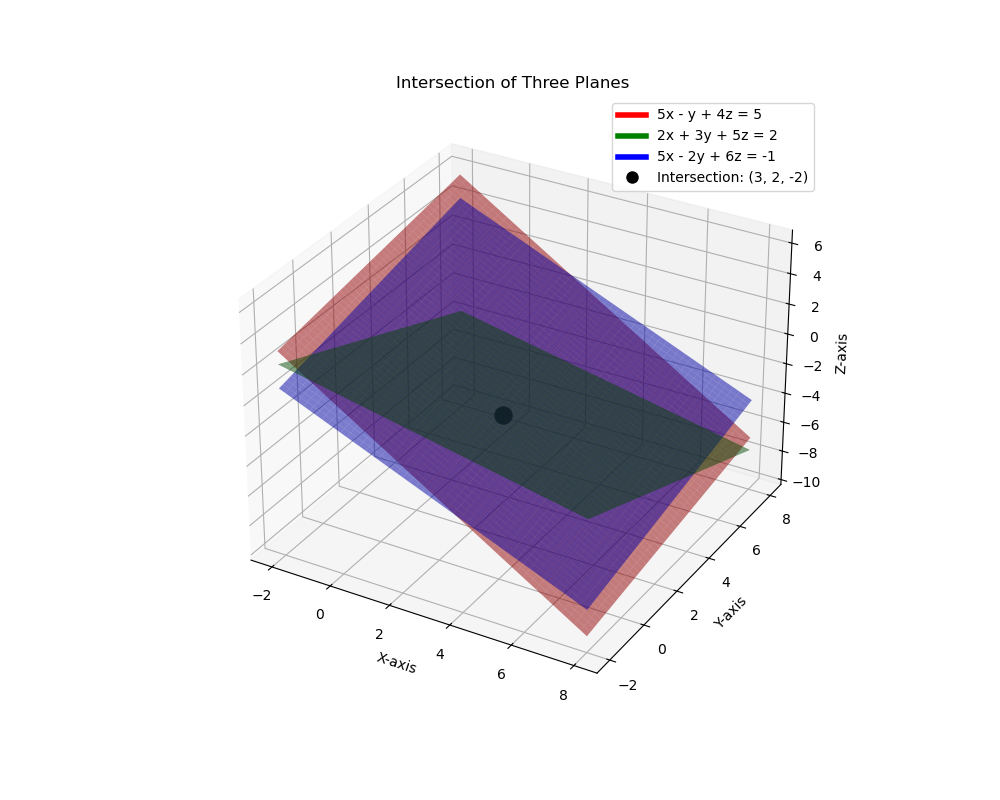
\includegraphics[width=0.7\columnwidth]{figs/Figure_1.png}
    \label{fig:placeholder}
    \caption{}
\end{figure}
\end{frame}
\end{document}
